\documentclass[12pt,a4paper]{article}
%\usepackage{ctex}
\usepackage{amsmath,amscd,amsbsy,amssymb,latexsym,url,bm,amsthm}
\usepackage{epsfig,graphicx,subfigure}
\usepackage{enumitem,balance}
\usepackage{wrapfig}
\usepackage{mathrsfs,euscript}
\usepackage[usenames]{xcolor}
\usepackage{here}
\usepackage{hyperref}
\usepackage[vlined,ruled,linesnumbered]{algorithm2e}
\usepackage{array}
\hypersetup{colorlinks=true,linkcolor=black}

\newtheorem{theorem}{Theorem}
\newtheorem{lemma}[theorem]{Lemma}
\newtheorem{proposition}[theorem]{Proposition}
\newtheorem{corollary}[theorem]{Corollary}
\newtheorem{exercise}{Exercise}
\newtheorem*{solution}{Solution}
\newtheorem{definition}{Definition}
\theoremstyle{definition}

\renewcommand{\thefootnote}{\fnsymbol{footnote}}

\newcommand{\postscript}[2]
 {\setlength{\epsfxsize}{#2\hsize}
  \centerline{\epsfbox{#1}}}

\renewcommand{\baselinestretch}{1.0}

\setlength{\oddsidemargin}{-0.365in}
\setlength{\evensidemargin}{-0.365in}
\setlength{\topmargin}{-0.3in}
\setlength{\headheight}{0in}
\setlength{\headsep}{0in}
\setlength{\textheight}{10.1in}
\setlength{\textwidth}{7in}
\makeatletter \renewenvironment{proof}[1][Proof] {\par\pushQED{\qed}\normalfont\topsep6\p@\@plus6\p@\relax\trivlist\item[\hskip\labelsep\bfseries#1\@addpunct{.}]\ignorespaces}{\popQED\endtrivlist\@endpefalse} \makeatother
\makeatletter
\renewenvironment{solution}[1][Solution] {\par\pushQED{\qed}\normalfont\topsep6\p@\@plus6\p@\relax\trivlist\item[\hskip\labelsep\bfseries#1\@addpunct{.}]\ignorespaces}{\popQED\endtrivlist\@endpefalse} \makeatother

\begin{document}
\noindent

%========================================================================
\noindent\framebox[\linewidth]{\shortstack[c]{
\Large{\textbf{Lab08-Graph Exploration}}\vspace{1mm}\\
CS214-Algorithm and Complexity, Xiaofeng Gao \& Lei Wang, Spring 2021.}}
\begin{center}
\footnotesize{\color{red}$*$ If there is any problem, please contact TA Yihao Xie. }

\footnotesize{\color{blue}$*$ Name:Beichen Yu  \quad Student ID:519030910245 \quad Email: polarisybc@sjtu.edu.cn}
\end{center}

\begin{enumerate}

	\item Given a graph $G = (V, E)$. Prove the following propositions.
	
	\begin{enumerate}
		\item Let $e$ be a maximum-weight edge on some cycle of connected graph $G=(V,E)$.
        Then there is a minimum spanning tree of $G$ that does not include $e$. Moreover, there is no minimum spanning tree of $G$ that includes $e$ if $e$ is the unique maximum-weight edge on the cycle. 
		\item Let $T$ and $T'$ are two different minimum spanning trees of $G$. Then $T'$ can be obtained from $T$ by repeatly substitute one edge in $T\backslash T'$ by one edge in $T'\backslash T$ and meanwhile the result after each subsitution is still a minimum spanning tree.
	\end{enumerate}
	
	\begin{solution}
	\begin{enumerate}
	\item It is obvious that in a circle has $n$ edges, in the spanning tree we must delete at least one edge to confirm that there is only one path between any two vertices. So in that circle, we must choose at least one edge to delete. Because $e$ is the maximum-weight edge, to get a minimum spanning tree, there is no better way than delete $e$, so begin with deleting $e$ we can get a minimum spanning tree without $e$. Moreover, if $e$ is the unique maximum-weight edge on the cycle, deleting $e$ is the only optimal solution to get a minimum spanning tree, so there is no minimum spanning tree that includes $e$.
	
	\item Assume that there are $n$ edges in the minimal spanning tree. Denote $ w(e) $ as the weight of edge $ e $. 
	Assume $ a_{1}, a_{2}, \cdots, a_{n} $ are edges of $ T $, and  $ b_{1}, b_{2}, \cdots, b_{n} $ are edges of $ T^{\prime} $. And assume that $ w(a_{1}) \leqslant w(a_{2}) \leqslant \cdots \leqslant w(a_{n}); w(b_{1}) \leqslant w(b_{2}) \leqslant \cdots \leqslant w(b_{n}) $. 

	Assume $ i $ is the first time that $ w(a_i) \neq w(b_i) $. And assume that $ w(a_i) \geqslant w(b_i) $.

	In the first case, $ b_{i} \in T $. Because $ \forall t < i : w(a_{t}) = w(b_{t}) $, we can confirm that $ \exists j>i $ and $ w(a_{j}) = w(b_{i}) $. So $ w(b_{i}) = w(a_{j}) \geqslant w(a_{i}) \geqslant w(b_{i})$. That means $ w(a_{i}) = w(b_{i}) $.

	In the second case, $ b_{i} \notin T $. If we add $ b_{i} $ into $ T $, it will form a circle somewhere. Obviously, there is an edge $ a_{j} \notin T^{\prime}$ and $j \geqslant i$. Because $ T $ is a minimal spanning tree, $ w(b_{i}) $ is bigger or equal to the weight of any edge in that circle. So we have $ a_{j} \leqslant b_{i} $. So $ w(b_{i}) \leqslant w(a_{i})  \leqslant w(a_{j}) \leqslant w(b_{i})$. That means $ w(a_{i}) = w(b_{i}) $.

	So we confirm that $ w(a_{1}) = w(b_{1}), w(a_{2}) = w(b_{2}), \cdots, w(a_{n}) = w(b_{n}) $. That means $ T^\prime $ can be obtainedby recursively substitute one edge in $ T $ by one edge in $ T^\prime $.
	
	\end{enumerate}
	\end{solution}

    \item Let $G=(V,E)$ be a connected, undirected graph. Give an $O(|V|+|E|)$-time algorithm
    to compute a path in $G$ that traverses each edge in $E$ exactly once in each direction. Describe how you can find your way out of a maze if you are given a large supply of pennies.

	\begin{solution}
		We use an algorithm similar to the DFS. 
		
		We need a stack to store some information.

		At the beginning, all of the edges are not signed. 
		
		First, we choose a vertex to begin. We randomly choose an edge connected with the vertex, sign it with the out direction and push the edge into the stack. 
		
		Then we go to the next vertex. We do the \textbf{going-out operation}: just choose a never signed edge connected with the vertex, sign it with the out direction and push the edge into the stack.

		Repeat this operation until finding a vertex that all edges connected with it are signed.Then we do the \textbf{going-back operation}: we should pop the stack, and go back along the edge poped from the stack. Sign the edge with the back direction. Then we go back to the last vertex.
		
		If we can find a never signed edge connected with that vertex, repeat the \textbf{going-out operation}. Otherwise, repeat the \textbf{going-back operation}. Finally, we will go back to the origin vertex, and we find a path in $ G $ that traverses each edge in $ E $ exactly once in each direction.
	\end{solution}

    \item Consider the maze shown in Figure \ref{Fig-Maze}. The black blocks in the figure are blocks that can not be passed through. Suppose the block are explored in the order of right, down, left and up. That is, to go to the next block from $(X,Y)$, we always explore $(X,Y+1)$ first, and then $(X+1,Y)$,$(X,Y-1)$ and$(X-1,Y)$ at last. Answer the following subquestions:
    \begin{enumerate}
        \item Give the sequence of the blocks explored by using DFS to find a path from the "start" to the "finish".
        \item Give the sequence of the blocks explored by using BFS to find the \underline{shortest} path from the "start" to the "finish".
        \item Consider a maze with a larger size. Discuss which of BFS and DFS will be used to find one path and which will be used to find the shortest path from the start block to the finish block.
    \end{enumerate}
    
    \begin{figure}[H]
	\centering
	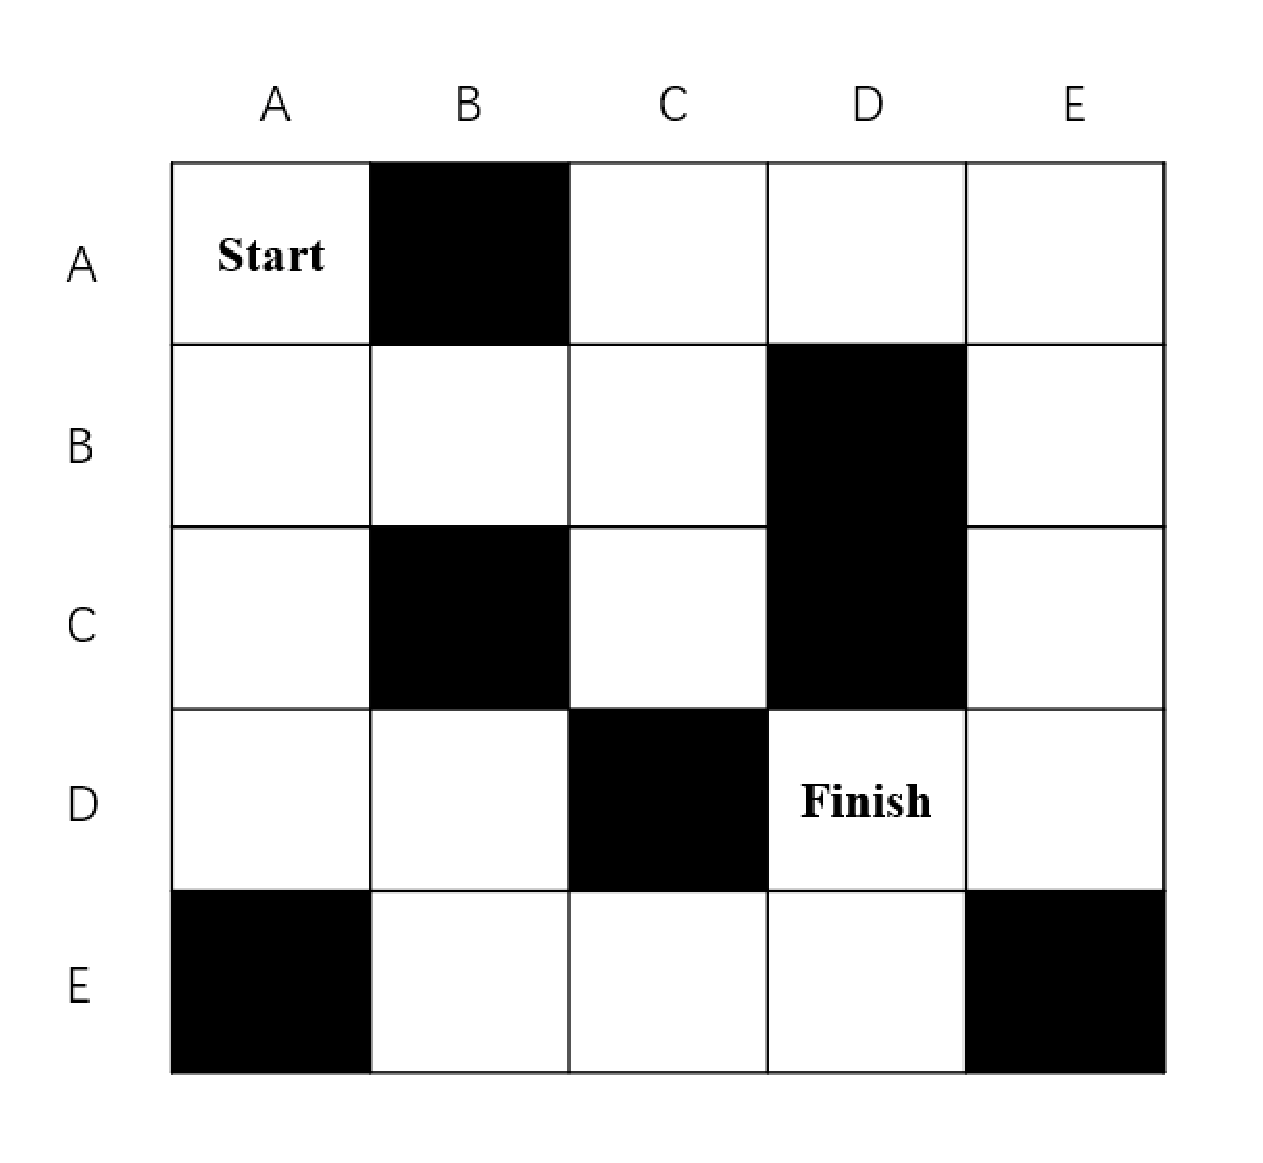
\includegraphics[width=0.3\textwidth]{Fig-Maze.pdf}
	\caption{An example of making room for one new element in the set of arrays.}
	\label{Fig-Maze}
	\end{figure}
	
	\begin{solution}
		\begin{enumerate}
			\item $ (A,A) \rightarrow (A,B) \rightarrow (A,C) \rightarrow (A,D) \rightarrow (B,D) \rightarrow (B,E) \rightarrow (C,E) \rightarrow (D,E) \rightarrow (D,D)$.
			\item $ (A,A) \rightarrow (A,B) \rightarrow (A,C) \rightarrow (B,B) \rightarrow (A,D) \rightarrow (C,B) \rightarrow (B,D) \rightarrow (C,C) \rightarrow (C,A) \rightarrow (B,E) \rightarrow (D,A) \rightarrow (C,E) \rightarrow (E,A) \rightarrow (D,E) \rightarrow (E,B) \rightarrow (D,D) $
			
			The shortest path from the ``start" to the ``finish" is the same as the result of DFS algorithm:  $ (A,A) \rightarrow (A,B) \rightarrow (A,C) \rightarrow (A,D) \rightarrow (B,D) \rightarrow (B,E) \rightarrow (C,E) \rightarrow (D,E) \rightarrow (D,D)$.
			\item If the maze is larger, BFS is a better algorithm. Using DFS, we can search only one path once.  If we can't find the ``finish'', we have go back to the original position. Besides, if using DFS, the number of recursion levels will be very deep. If using BFS, we can approach the ``finish'' step by step. The larger the maze is, the more efficient BFS is.
		\end{enumerate}
	\end{solution}
	\item Given a directed graph $G$, whose vertices and edges information are introduced in data file "SCC.in". Please find its number of Strongly Connected Components with respect to the following subquestions.
    
    \begin{enumerate}
    	\item Read the code and explanations of the provided C/C++ source code "SCC.cpp", and try to complete this implementation.
    	\item Visualize the above selected Strongly Connected Components for this graph $G$. Use the $Gephi$ or other software you preferred to draw the graph. {\color{blue}(If you feel that the data provided in ``SCC.in'' is not beautiful, you can also generate your own data with more vertices and edges than $G$ and draw an additional graph. Notice that results of your visualization will be taken into the consideration of Best Lab.)}
    \end{enumerate}	
	\begin{solution}
		\begin{enumerate}
			\item The .cpp code is included in the .zip file. And the answer is 202.
			\item Replace each strongly connected component with a vertex, and use the size and color of the vertex to represent the number of vertices in the original strongly connected component. Then use \textit{Gephi} to draw this figure.			
			\begin{figure}[H]
				\centering
				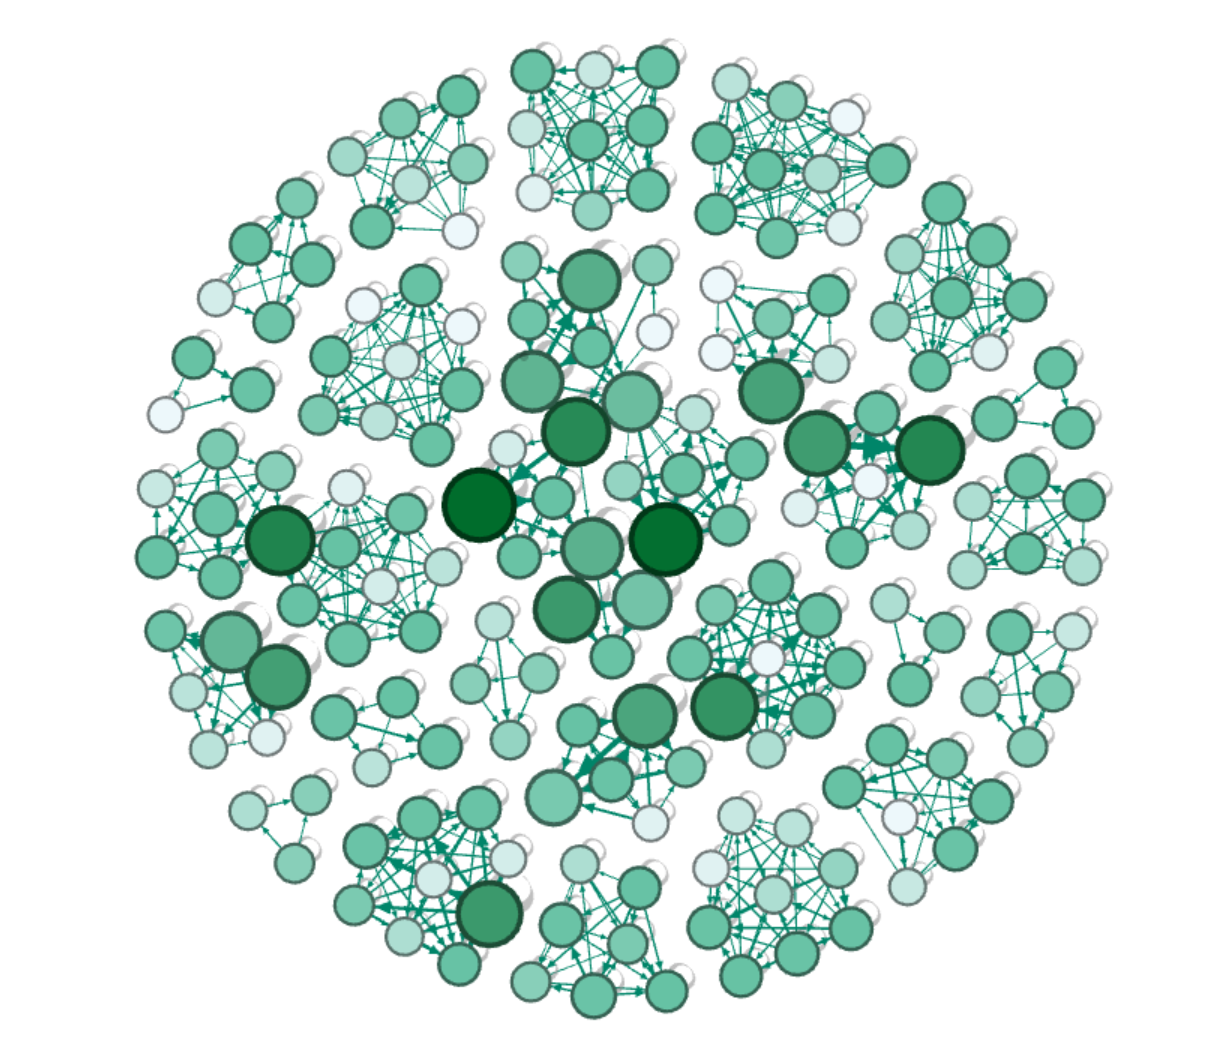
\includegraphics[width=0.65\textwidth]{scc.png}
				\caption{The Strongly Connected Components}
			\end{figure}
		\end{enumerate}
	\end{solution}
\end{enumerate}



\textbf{Remark:} Please include your .pdf, .tex, .cpp files for uploading with standard file names.
\newpage


%========================================================================
\end{document}